\newcommand{\coursepath}{/teaching/2021/ConcDisSys}
\newcommand{\courseurl}{\url{https://www.cst.cam.ac.uk\coursepath}}
\newcommand{\thisyear}{2020/21}

\begin{document}
\title{Distributed Systems}
\subtitle{University of Cambridge\\Computer Science Tripos, Part IB\\Michaelmas term \thisyear\\\courseurl}
        
\author{Dr.\ Martin Kleppmann\\mk428@cst.cam.ac.uk}
\date{}
\maketitle

\section{Introduction}

\begin{frame}
    \label{s:title}
    \begin{center}
        \textbf{\huge{\color{darkblue}{Distributed Systems}}} \\[2em]
        The second half of \emph{Concurrent and Distributed Systems}\\[0.5em]
        \courseurl\\[2em]
        Dr.\ Martin Kleppmann (mk428@cam) \\[0.5em]
        University of Cambridge \\[0.5em]
        Computer Science Tripos, Part IB \\[0.5em]
        Michaelmas term \thisyear \\[0.5em]
    \end{center}
\end{frame}

This 8-lecture course on distributed systems forms the second half of \emph{Concurrent and Distributed Systems}.
While the first half focussed on concurrency among multiple processes or threads running on the same computer, this second half takes things further by examining systems consisting of multiple communicating computers.

Concurrency on a single computer is also known as \emph{shared-memory concurrency}, since multiple threads running in the same process have access to the same address space.
Thus, data can easily be passed from one thread to another: a variable or pointer that is valid for one thread is also valid for another.

This situation changes when we move to distributed systems.
We still have concurrency in a distributed system, since different computers can execute programs in parallel.
However, we don't typically have shared memory, since each computer in a distributed system runs its own operating system with its own address space, using the memory built into that computer.
Different computers can only communicate by sending each other messages over a network.

(Limited forms of distributed shared memory exist in some supercomputers and research systems, and there are technologies like \emph{remote direct memory access} (RDMA) that allow computers to access each others' memory over a network.
Also, databases can in some sense be regarded as shared memory, but with a different data model compared to byte-addressable memory.
However, broadly speaking, most practical distributed systems are based on message-passing.)

Each of the computers in a distributed system is called a \emph{node}.
Here, ``computer'' is interpreted quite broadly: nodes might be desktop computers, servers in datacenters, mobile devices, internet-connected cars, industrial control systems, sensors, or many other types of device.
In this course we don't distinguish them: a node can be any type of communicating computing device.

\begin{frame}
    \label{s:dist-sys-definition}
    \frametitle{A distributed system is\dots}
    \begin{itemize}
        \item<1-> \emph{``{\dots}a system in which the failure of a computer you didn't even know existed can render your own computer unusable.''} --- Leslie Lamport\\[1em]
        \item<2> {\dots}multiple computers communicating via a network\dots
        \item<2> {\dots}trying to achieve some task together
        \item<2> Consists of ``nodes'' (computer, phone, car, robot, \dots)
    \end{itemize}
    \hfill\includegraphics<1>[height=4cm]{images/lamport.jpg}
\end{frame}
\inlineslide{s:dist-sys-definition}\label{l:dist-sys-definition}
% reference for Lamport quote: https://www.microsoft.com/en-us/research/publication/distribution/

\subsection{About this course}

These notes and the lecture recordings should be self-contained, but if you would like to read up on further detail, there are several suggested textbooks:
\begin{itemize}
    \item Maarten van Steen and Andrew S.\ Tanenbaum. \emph{Distributed Systems}. ISBN 978-1543057386.
        Free download from \url{https://www.distributed-systems.net/index.php/books/ds3/} (third edition, 2017).

        This book gives a broad overview over a large range of distributed systems topics, with lots of examples from practical systems.

    \item Christian Cachin, Rachid Guerraoui, and Luís Rodrigues.
        \emph{Introduction to Reliable and Secure Distributed Programming}.
        Second edition, Springer, 2011. ISBN 978-3-642-15259-7.

        Ebook download for Cambridge users: \url{https://link.springer.com/book/10.1007/978-3-642-15260-3} then click Log in $\rightarrow$ via Shibboleth $\rightarrow$ type \emph{University of Cambridge} $\rightarrow$ log in with Raven.

        This book is more advanced, going into depth on several important distributed algorithms, and proving their correctness.
        Recommended if you want to go deeper into the theory than covered in this course.

    \item Martin Kleppmann. \emph{Designing Data-Intensive Applications}, O'Reilly, 2017. ISBN 978-1449373320.

        This book goes more in the direction of databases, but also covers a number of distributed systems topics.
        It is designed for software engineers in industry working with distributed databases.

    \item Jean Bacon and Tim Harris. \emph{Operating Systems: Concurrent and Distributed Software Design}.
        Addison-Wesley, 2003. ISBN 978-0321117892.

        This book provides a link to the \emph{concurrent systems} half of the course, and to operating systems topics.
\end{itemize}

\begin{frame}
    \label{s:reading}
    \frametitle{Recommended reading}
    \begin{itemize}
        \item van Steen \& Tanenbaum.\\ ``\textbf{Distributed Systems}''\\(any ed), free ebook available
        \item Cachin, Guerraoui \& Rodrigues. \\ ``\textbf{Introduction to Reliable and Secure Distributed Programming}'' (2nd ed), Springer 2011
        \item Kleppmann.\\ ``\textbf{Designing Data-Intensive Applications}'',\\O’Reilly 2017
        \item Bacon \& Harris.\\ ``\textbf{Operating Systems: Concurrent and Distributed Software Design}'', Addison-Wesley 2003
    \end{itemize}
\end{frame}
\inlineslide{s:reading}

The syllabus, slides, and lecture notes for this course have been substantially revised for 2020/21.
This means that new mistakes may have crept in.
If you notice anything wrong, or if anything is unclear, please let the lecturer know by email (\url{mk428@cst.cam.ac.uk})!

As for other courses, past exam questions are available at \url{https://www.cl.cam.ac.uk/teaching/exams/pastpapers/t-ConcurrentandDistributedSystems.html}.
Because of syllabus changes, some of the past exam questions are no longer applicable.
TODO: details on which questions are obsolete.

This course is related to several other courses in the tripos, as shown on Slide~\ref{l:other-courses}.

\begin{frame}
    \label{s:other-courses}
    \frametitle{Relationships with other courses}
    \begin{itemize}
        \item \textbf{Concurrent Systems} -- Part IB\\
            (every distributed system is also concurrent)
        \item \textbf{Operating Systems} -- Part IA\\
            (inter-process communication, scheduling)
        \item \textbf{Databases} -- Part IA\\
            (many modern databases are distributed)
        \item \textbf{Computer Networking} -- Part IB Lent term\\
            (distributed systems involve network communication)
        \item \textbf{Further Java} -- Part IB Michaelmas\\
            (distributed programming practical exercises)
        \item \textbf{Security} -- Part IB Easter term\\
            (network protocols with encryption \& authentication)
        \item \textbf{Cloud Computing} -- Part II\\
            (distributed systems for processing large amounts of data)
    \end{itemize}
\end{frame}
\inlineslide{s:other-courses}\label{l:other-courses}


\subsection{Pros and cons of distributed systems}

There are a number of reasons for creating distributed systems.
Some applications are \emph{instrinsically distributed}: if you want to send a message from your phone to your friend's phone, that operation inevitably requires those phones to communicate via some kind of network.

Some distributed systems do things that in principle a single computer could do, but they do it \emph{more reliably}.
A single computer can fail and might need to be rebooted from time to time, but if you are using multiple nodes, then one node can continue serving users while another node is rebooting.
Thus, a distributed system has the potential to be more reliable than a single computer, at least if it is well-designed (somewhat contradicting Lamport's quote on Slide~\ref{l:dist-sys-definition})!

Another reason for distribution is for better \emph{performance}: if a service has users all over the world, and they all have to access a single node, then either the users in the UK or the users in New Zealand are going to find it slow (or both).
By placing nodes in multiple locations around the world, we can get around the slowness of the speed of light by routing each user to a nearby node.

Finally, some large-scale data processing or computing tasks are simply \emph{too big} to perform on a single computer, or would be intolerably slow.
For example, the Large Hadron Collider at CERN is supported by a worldwide computing infrastructure with 1 million CPU cores for data analysis, and 1 exabyte ($10^{18}$ bytes) of storage! See \url{https://wlcg-public.web.cern.ch/}.

\begin{frame}
    \label{s:why-distribute}
    \frametitle{Why make a system distributed?}
    \begin{itemize}\pause
        \item \textbf{It's inherently distributed:}\\e.g. sending a message from your mobile phone to your friend's phone\pause
        \item \textbf{For better reliability:}\\even if one node fails, the system as a whole keeps functioning\pause
        \item \textbf{For better performance:}\\get data from a nearby node rather than one halfway round the world\pause
        \item \textbf{To solve bigger problems:}\\e.g. huge amounts of data, can't fit on one machine
    \end{itemize}
\end{frame}
\inlineslide{s:why-distribute}

However, there are also downsides to distributed systems, because things can go wrong, and the system needs to deal with such faults.
The network may fail, leaving the nodes unable to communicate.

\begin{frame}
    \label{s:no-internet}
    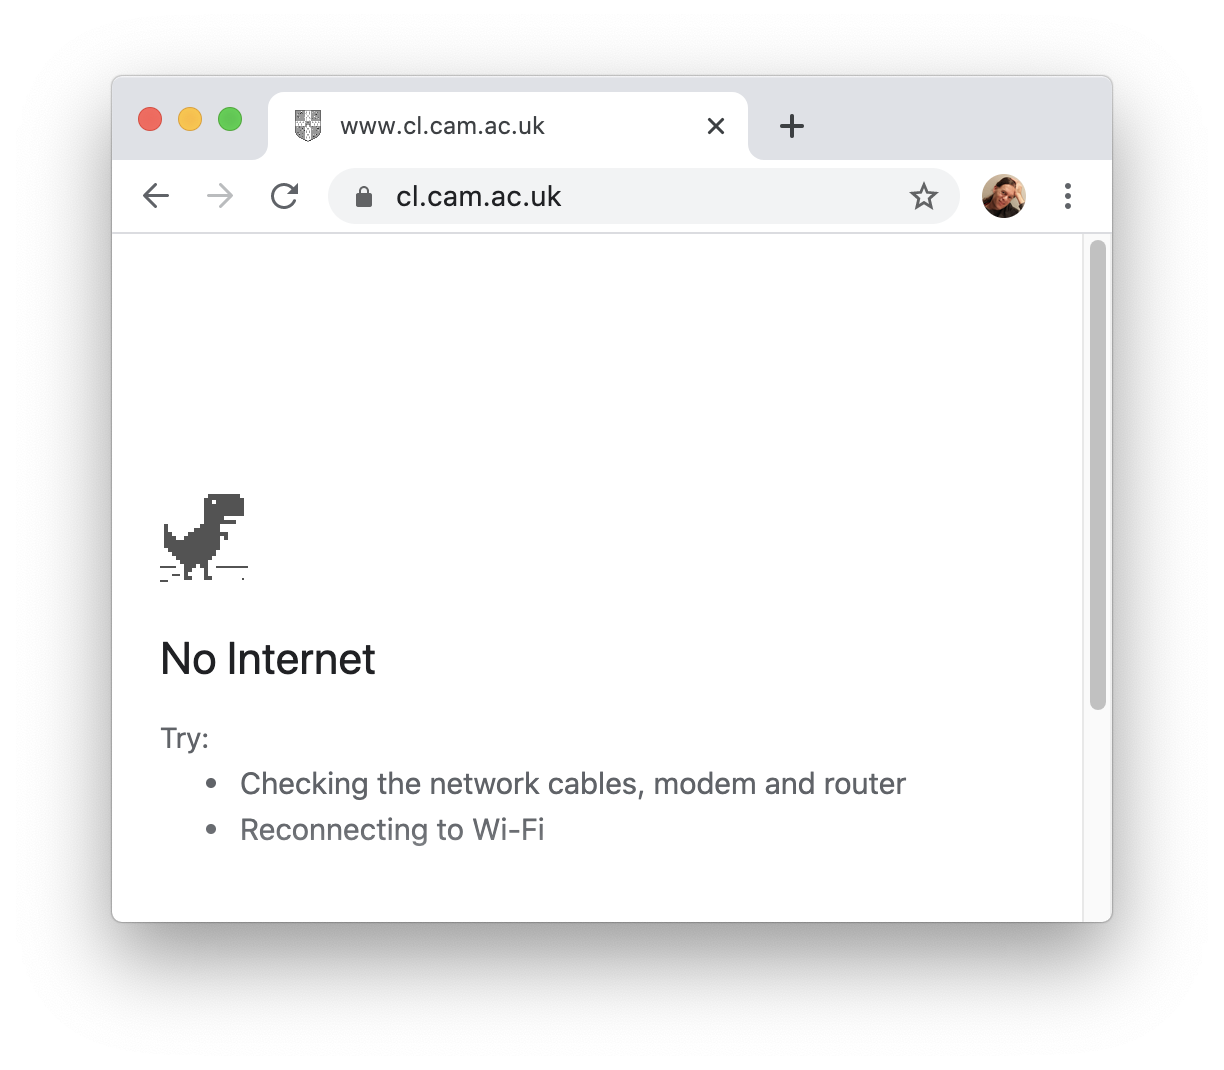
\includegraphics[height=\paperheight]{images/no-internet.png}
\end{frame}
\inlineslide{s:no-internet}

Another thing that can go wrong is that a node may crash, or run much slower than usual, or misbehave in some other way (perhaps due to a software bug or a hardware failure).
If we want one node to take over when another node crashes, we need to detect that a crash has happened; as we shall see, even that is not straightforward.
Network failures and node failures can happen at any moment, without warning.

In a single computer, if one component fails (e.g.\ one of the RAM modules develops a fault), we normally don't expect the computer to continue working nevertheless: it will probably just crash.
Software does not need to be written in a way that explicitly deals with faulty RAM.
However, in a distributed system we often \emph{do} want to tolerate some parts of the system being broken, and for the rest to continue working.
For example, if one node has crashed (a \emph{partial failure}), the remaining nodes may still be able to continue providing the service.

If one component of a system stops working, we call that a \emph{fault}, and many distributed systems strive to provide \emph{fault tolerance}: that is, the system as a whole continues functioning despite the fault.
Dealing with faults is what makes distributed computing fundamentally different, and often harder, compared to programming a single computer.
Some distributed system engineers believe that if you can solve a problem on a single computer, it is basically easy!
Though, in fairness to our colleagues in other areas of computer science, this is probably not true.

\begin{frame}
    \label{s:why-not}
    \frametitle{Why NOT make a system distributed?}
    The trouble with distributed systems:
    \begin{itemize}
        \item Communication may fail (and we might not even know it has failed).
        \item Processes may crash (and we might not know).
        \item All of this may happen nondeterministically.
    \end{itemize}\vspace{1em}\pause
    \textbf{Fault tolerance}: we want the system as a whole to continue working, even when some parts are faulty.\\[1em]
    This is hard.\\[1em]
    Writing a program to run on a single computer is comparatively easy?!
\end{frame}
\inlineslide{s:why-not}


\subsection{Distributed systems and computer networking}

When studying distributed systems, we usually work with a high-level abstraction of the hardware.

\begin{frame}
    \label{s:networking}
    \frametitle{Distributed Systems and Computer Networking}
    We use a simple abstraction of communication:
    \begin{center}
        \begin{tikzpicture}
            \node [circle,fill=red!10,draw] (i) at (0,0) {node $i$};
            \node [circle,fill=red!10,draw] (j) at (6,0) {node $j$};
            \draw [bigarrow] (i) -- node [above] {message $m$} (j);
        \end{tikzpicture}
    \end{center}

    Reality is much more complex:
    \begin{itemize}
        \item \textbf{Various network operators:}\\ eduroam, home DSL, cellular data, coffee shop wifi, submarine cable, satellite\dots\\[1em]
        \item \textbf{Physical communication:}\\ electric current, radio waves, laser, hard drives in a van\dots
    \end{itemize}
\end{frame}
\inlineslide{s:networking}

In this course, we just assume that there is some way for one node to send a message to another node.
We don't particularly care how that message is physically represented or encoded~-- the network protocols, informally known as the \emph{bytes on the wire}~-- because the basic principle of sending and receiving messages remains the same, even as particular networking technologies come and go.
The ``wire'' may actually be radio waves, lasers, a USB thumb drive in someone's pocket, or even hard drives in a van.

\begin{frame}[plain]
    \label{s:snowball}
    \frametitle{Hard drives in a van?!}
    \begin{center}
        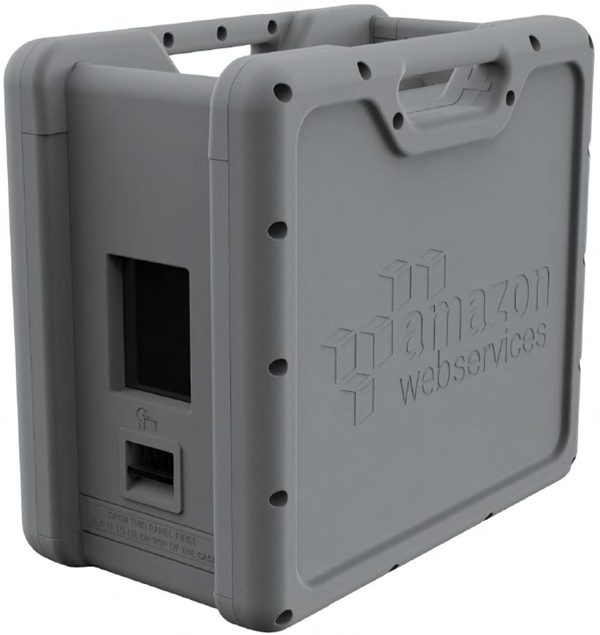
\includegraphics[height=5cm]{images/aws-snowball.png}\\[0.5em]
        \footnotesize{\url{https://docs.aws.amazon.com/snowball/latest/ug/using-device.html}}
    \end{center}
\end{frame}
\inlineslide{s:snowball}

Indeed, if you want to send a very large message (think tens of terabytes), it would be slow to send that data over the Internet, and it is in fact faster to write that data to a bunch of hard drives, load them into a van, and to drive them to their destination.
But from a distributed systems point of view, the method of delivering the message is not important: we only see an abstract communication channel with a certain \emph{latency} (delay from the time a message is sent until it is received) and \emph{bandwidth} (the volume of data that can be transferred per unit time).

The Computer Networking course in Lent term focusses on the network protocols that enable messages to get to their destination.
The study of distributed systems builds upon that facility, and instead focusses on how several nodes should coordinate in order to achieve some shared task.
The design of distributed algorithms is about deciding what messages to send, and how to process the messages when they are received.

\subsection{Example: the web, a client-server distributed system}

The web is an example of a distributed system that you use every day.

\begin{frame}[plain]
    \label{s:website}
    \begin{tikzpicture}[remember picture,overlay]
        \node at (current page.center) {
\includegraphics[height=\paperheight]{images/website.png}};
    \end{tikzpicture}
\end{frame}
\inlineslide{s:website}

In the web there are two main types of nodes: \emph{servers} host websites, and \emph{clients} (web browsers) display them.
When you load a web page, your web browser sends a \emph{HTTP request} message to the appropriate server.
On receiving that request, the web server sends a \emph{response} message containing the page contents to the client that requested it.

\begin{frame}
    \label{s:client-server}
    \frametitle{Client-server example: the web}
    Time flows from top to bottom.
    \begin{center}
        \begin{tikzpicture}
            \node [rectangle,fill=red!10,draw] (client) at (0,4) {client};
            \node [rectangle,fill=red!10,draw] (server) at (8,4) {server www.cst.cam.ac.uk};
            \draw (client) -- (0,0);
            \draw (server) -- (8,0);
            \draw<2-> [bigarrow,thick] (0,3) -- node [above,sloped] {GET \coursepath} (8,2);
            \draw<3> [bigarrow,thick] (8,1.5) -- node [above,sloped] {\texttt{<!DOCTYPE html><html>...}} (0,0.5);
        \end{tikzpicture}
    \end{center}
\end{frame}
\inlineslide{s:client-server}

\begin{frame}[plain]
    \label{s:http-capture}
    \begin{tikzpicture}
        \node at (0,0) {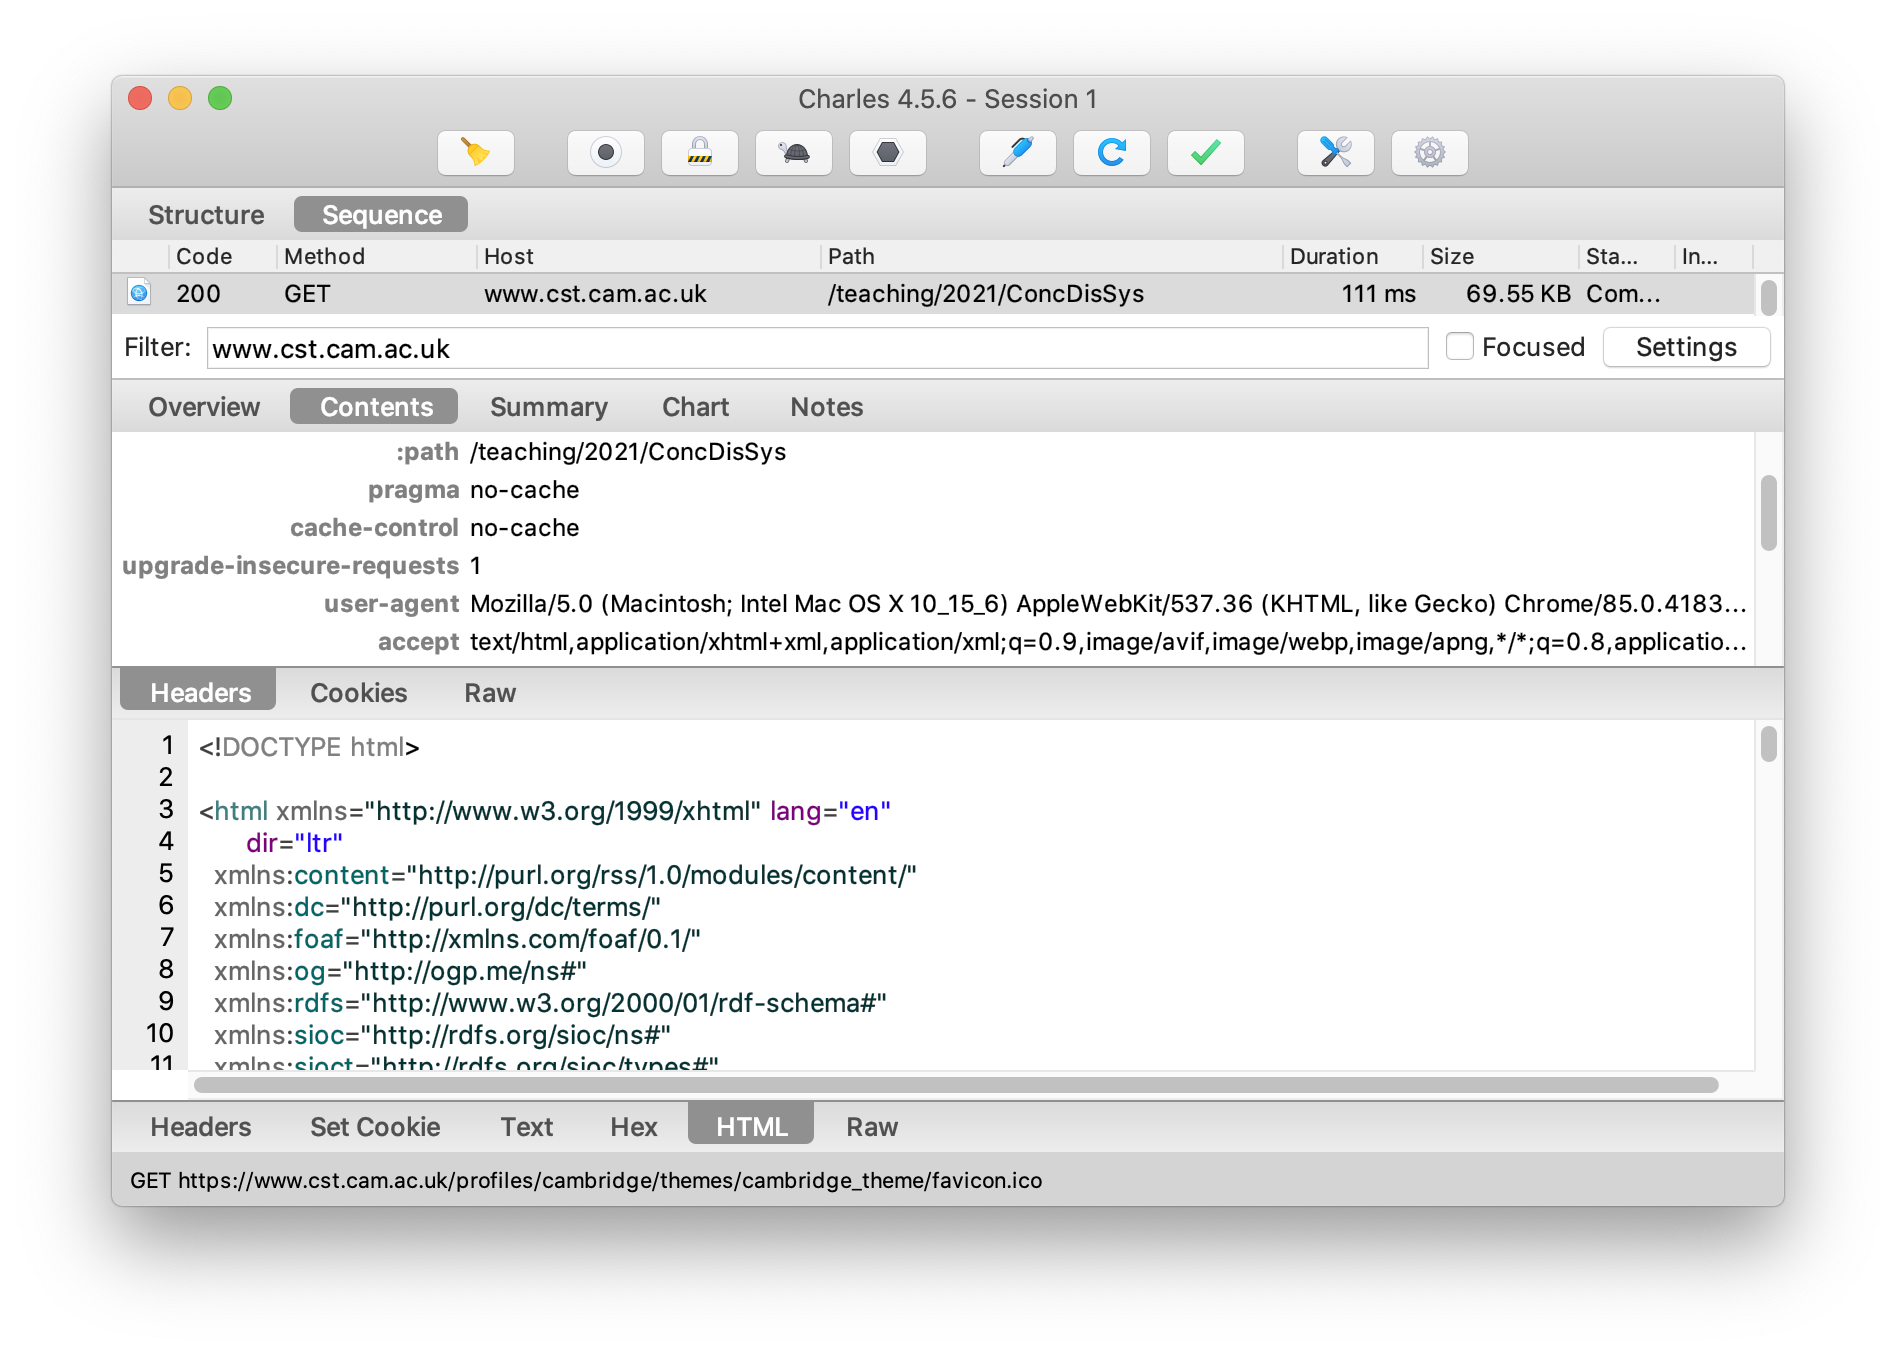
\includegraphics[height=8cm]{images/http-capture.png}};
        \node<2> (request) at (-4,-4.5) [red] {request message};
        \node<2> (response) at (2,-4.5) [red] {response message};
        \draw<2> [-Stealth,red,line width=4pt] (request) -- (-4,0.5);
        \draw<2> [-Stealth,red,line width=4pt] (response) -- (0,-1.2);
    \end{tikzpicture}
\end{frame}
\inlineslide{s:http-capture}\label{l:http-capture}

These messages are normally invisible, but we can capture and visualise the network traffic with a tool such as Charles (\url{https://www.charlesproxy.com/}), shown on Slide~\ref{l:http-capture}.

% TODO live demo: launch Charles and then run
% curl -kx localhost:8888 https://www.cst.cam.ac.uk/teaching/2021/ConcDisSys/
% Also show how in Wireshark it breaks down into lots of small packets, with filter:
% ip.addr == 128.232.132.21

In a URL such as \courseurl, the part of the URL between the \verb|//| and the following \verb|/| is the hostname of the server to which the client is going to send the request (\texttt{www.cst.cam.ac.uk}), and the rest (\texttt{\coursepath}) is the path that the client asks for in its request message.
Besides the path, the request also contains some extra information, such as the version of the client software (the \emph{user-agent}), and a list of file formats that the client understands (the \emph{accept header}).
The response message contains the file that was requested, and an indicator of its file format (the \emph{content-type}); in the case of a web page, this might be a HTML document, an image, a video, a PDF document, or any other type of file.

Since the requests and responses can be larger than we can fit in a single network packet, the HTTP protocol runs on top of TCP, which breaks down a large chunk of data into a stream of small network packets (see Slide~\ref{l:wireshark}), and puts them back together again at the recipient.
HTTP also allows multiple requests and multiple responses to be sent over a single TCP connection.
However, when looking at this protocol from a distributed systems point of view, this detail is not important: we treat the request as one message and the response as another message, regardless of the number of physical network packets involved in transmitting them.
This keeps things independent of the underlying networking technology.

\begin{frame}<article:0>[plain]
    \label{s:wireshark}
    \begin{tikzpicture}[remember picture,overlay]
        \node at (current page.center) {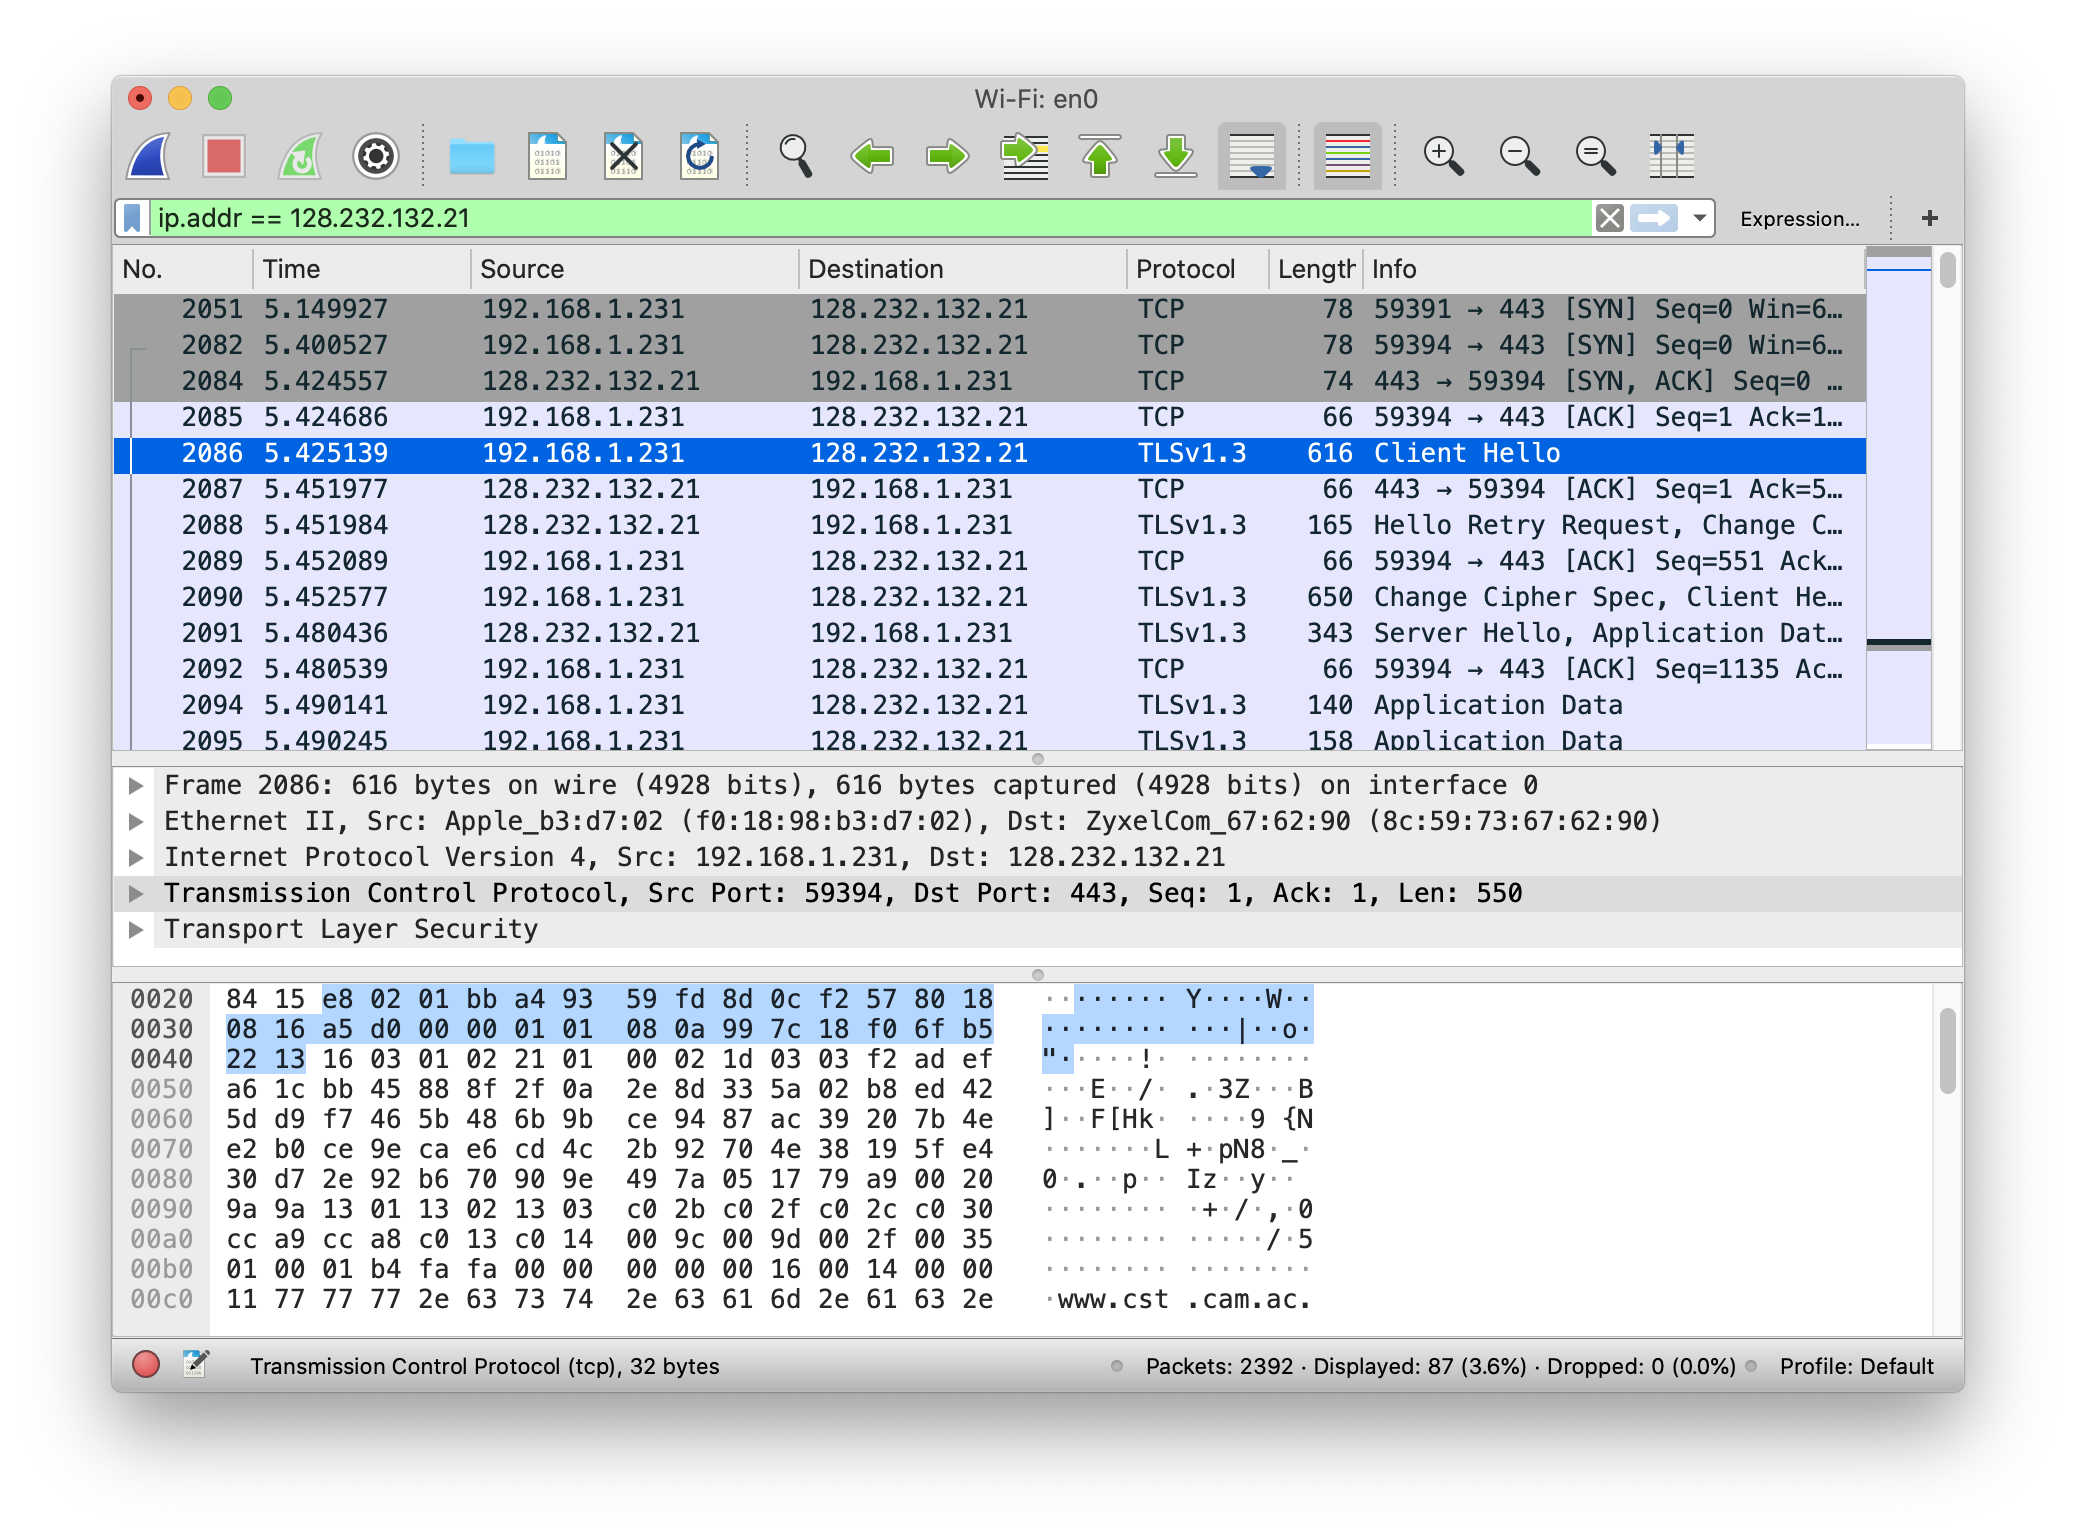
\includegraphics[height=\paperheight]{images/wireshark.png}};
    \end{tikzpicture}
\end{frame}
\inlineslide{s:wireshark}\label{l:wireshark}

\subsection{Example: remote procedure calls (RPC)}

Another example of an everyday distributed system is when you buy something online using a credit/debit card.
When you enter your card number in some online shop, that shop will send a payment request over the Internet to a service that specialises in processing card payments.

\begin{frame}
    \label{s:payment-example}
    \frametitle{Client-server example: online payments}
    \begin{center}
        \begin{tikzpicture}
            \node [rectangle,fill=red!10,draw] (client) at (0,4) {online shop};
            \node [rectangle,fill=red!10,draw] (server) at (8,4) {payments service};
            \draw (client) -- (0,0);
            \draw (server) -- (8,0);
            \draw<2-> [bigarrow,thick] (0,3) -- node [above,sloped] {charge {\textsterling}3.99 to credit card 1234\dots} (8,2);
            \draw<3> [bigarrow,thick] (8,1.5) -- node [above,sloped] {success} (0,0.5);
        \end{tikzpicture}
    \end{center}
\end{frame}
\inlineslide{s:payment-example}

The payments service in turn communicates with a card network such as Visa or MasterCard, which communicates with the bank that issued your card in order to take the payment.

For the programmers who are implementing the online shop, the code for processing the payment may look something like the code on Slide~\ref{l:payment-rpc}.

\begin{frame}
    \label{s:payment-rpc}
    \frametitle{Remote Procedure Call (RPC) example}
    \inputminted{java}{code/payment-rpc.java}
    \begin{tikzpicture}[remember picture,overlay]
        \node (call) [xshift=2cm,yshift=-0.5cm] at (current page.center) {};
        \node<2> (label) [anchor=south east,red,yshift=0.5cm] at (current page.south east) {Implementation of this function is on another node!};
        \draw<2> [-Stealth,red,line width=4pt] (label) -- (call);
    \end{tikzpicture}
\end{frame}
\inlineslide{s:payment-rpc}\label{l:payment-rpc}

Calling the \verb|processPayment| function looks like calling any other function, but in fact, what is happening behind the scenes is that the shop is sending a request to the payments service, waiting for a response, and then returning the response it received.
The actual implementation of \verb|processPayment|~-- the logic that communicates with the card network and the banks~-- does not exist in the code of the shop: it is part of the payments service, which is another program running on another node belonging to a different company.

This type of interaction, where code on one node appears to call a function on another node, is called a \emph{Remote Procedure Call} (RPC).
In Java, it is called \emph{Remote Method Invocation} (RMI).
The software that implements RPC is called an \emph{RPC framework} or \emph{middleware}.
(Not all middleware is based on RPC; there is also middleware that uses different communication models.)

When an application wishes to call a function on another node, the RPC framework provides a \emph{stub} in its place.
The stub has the same type signature as the real function, but instead of executing the real function, it encodes the function arguments in a message and sends that message to the remote node, asking for that function to be called.
The process of encoding the function arguments is known as \emph{marshalling}.
In the example on Slide~\ref{l:payment-json}, a JSON encoding is used for marshalling, but various other formats are also used in practice.

\begin{frame}[plain]
    \label{s:payment-json}
    \hspace*{-1cm}
    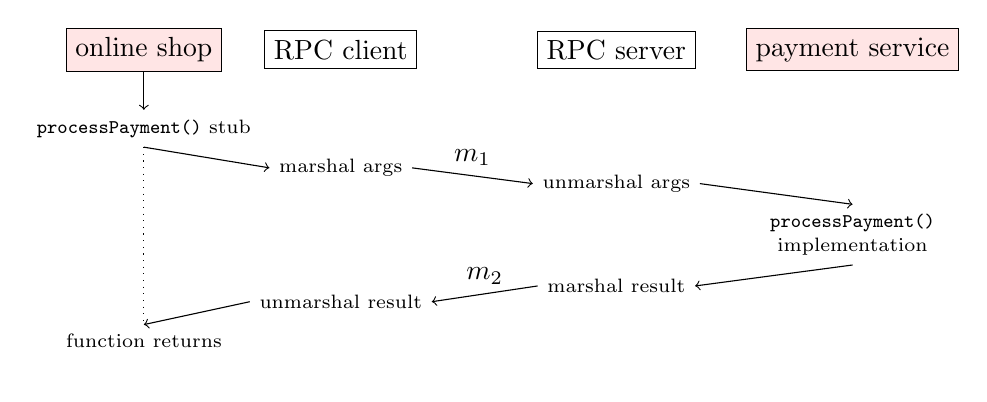
\begin{tikzpicture}
        \node [rectangle,fill=red!10,draw] (client) at (0,4) {online shop};
        \node [rectangle,draw] (rpc-client) at (2.5,4) {RPC client};
        \node [rectangle,draw] (rpc-server) at (6,4) {RPC server};
        \node [rectangle,fill=red!10,draw] (server) at (9,4) {payment service};
        \node [font=\scriptsize] (invoke) at (0,3) {\texttt{processPayment()} stub};
        \draw [->] (client) -- (invoke);
        \node<2-> [font=\scriptsize] (send-req) at (2.5,2.5) {marshal args};
        \draw<2-> [->] (invoke.south) -- (send-req.west);
        \node<2-> [font=\scriptsize] (recv-req) at (6,2.3) {unmarshal args};
        \draw<2-> [->] (send-req.east) -- node [above] {$m_1$} (recv-req.west);
        \node<3-> [font=\scriptsize] (exec) at (9,1.8) {\texttt{processPayment()}};
        \node<3-> [font=\scriptsize] (exec2) at (9,1.5) {implementation};
        \draw<3-> [->] (recv-req.east) -- (exec.north);
        \node<4-> [font=\scriptsize] (send-res) at (6,1) {marshal result};
        \draw<4-> [->] (exec2.south) -- (send-res.east);
        \node<4-> [font=\scriptsize] (recv-res) at (2.5,0.8) {unmarshal result};
        \draw<4-> [->] (send-res.west) -- node [above] {$m_2$} (recv-res.east);
        \node<5> [font=\scriptsize] (return) at (0,0.3) {function returns};
        \draw<5> [->] (recv-res.west) -- (return.north);
        \draw [dotted] (invoke.south) -- (0,0.5);
        \node at (0,0) {}; % so that messages below stay put as the slide builds
    \end{tikzpicture}
    \hspace*{-1cm}\mbox{
        \onslide<2->{
            $m_1$ = \begin{minipage}{5.5cm}
            \inputminted[fontsize=\scriptsize,frame=single,bgcolor=lightgrey]{json}{code/payment-rpc.json}
            \end{minipage}
        }
        \onslide<4->{
            $m_2$ = \begin{minipage}{3.8cm}
            \inputminted[fontsize=\scriptsize,frame=single,bgcolor=lightgrey]{json}{code/payment-response.json}
            \end{minipage}
        }
    }
\end{frame}
\inlineslide{s:payment-json}\label{l:payment-json}

The sending of the message from the RPC client to the RPC server may happen over HTTP (in which case this is also called a \emph{web service}), or one of a range of different network protocols may be used.
On the server side, the RPC framework unmarshals (decodes) the message and calls the desired function with the provided arguments.
When the function returns, the same happens in reverse: the function's return value is marshalled, sent as a message back to the client, unmarshalled by the client, and returned by the stub.
Thus, to the caller of the stub, it looks as if the function had executed locally.

\begin{frame}
    \label{s:rpc-discussion}
    \frametitle{Remote Procedure Call (RPC)}
    Ideally, RPC makes a call to a remote function look the same as a local function call.\\[1em]
    \textbf{``Location transparency''}:\\ system hides where a resource is located.\\[1em]\pause
    In practice\dots
    \begin{itemize}
        \item what if the service crashes during the function call?
        \item what if a message is lost?
        \item what if a message is delayed?
        \item if something goes wrong, is it safe to retry?
    \end{itemize}
\end{frame}
\inlineslide{s:rpc-discussion}

\supervision{
    Networks and nodes might fail.
    What are the implications for code that calls another node through RPC?
    How is RPC different from a local function call?
}{
    \begin{itemize}
        \item RPCs may time out if the request or response message is lost.
            Even if we retry, there is no guarantee that the messages will get through.
            The application must handle this error condition, and the possibility of failure may need to be reflected in the type signature.
            For example, JavaScript RPC clients often return a \emph{promise}, which can either succeed or fail.
        \item If a timeout occurs, the RPC client doesn't know whether the server executed the function; local function calls don't have this uncertainty.
        \item RPC is often much slower than a local function call, due to network latency.
        \item RPC clients and servers may need to take measures to make function invocation idempotent, to allow safe retries in case of message loss.
    \end{itemize}
}

% If the client sends the RPC request but receives no response, it doesn't know whether or not the server received and processed the request.
% It could resend the request if it doesn't hear back for a while, but that might cause the request to be performed more than once (e.g.\ charging a credit card twice), unless we take care to make the request idempotent.
% But even if we retry, there is no guarantee that the retried messages will get through either.
%
% Waiting forever is not a good approach, so in practice we have to give up after some timeout.
% As the client has not received a response, the RPC stub will not be able to return a value of the function's return type, but rather it will need to somehow indicate to the calling code that a timeout occurred, e.g.\ by throwing an exception.


Object-oriented middleware.

gRPC, Thrift, Java RMI, CORBA


Service-oriented architecture/microservices

\section{Models of distributed systems}

Fundamental abstraction: nodes (or processes); sending a message from one node to another.
A \emph{system model} captures our assumptions about how nodes and the network behave.

Faults and failures; fault tolerance; single point of failure

Availability (``five nines''), eg. online shop wants to be able to sell stuff 24/7; downtime = losing money

SLA: eg. 99\% of requests receive a successful response in less than 500 ms

``reliability'' of TCP; screenshots of network error + request timeout

Why distribute?
- Inherently distributed: communication, collaboration (Facebook, google docs).
- Scale, performance, fault tolerance

It's easy if you can do it on one machine! Don't distribute unless you have to. 

Distributed systems are fascinating because we have to work with partial knowledge and uncertain
truths. We never have certainty about the state of the system, because by the time we hear about
something, that state may already be outdated. In this way it resembles real life more than most of
computing! In real life you need to often make decisions with incomplete information.

Two generals problem, Byzantine generals problem
% two generals: https://link.springer.com/chapter/10.1007/3-540-08755-9_9

% network cable unplugged (image)
% sharks bite submarine cables https://slate.com/technology/2014/08/shark-attacks-threaten-google-s-undersea-internet-cables-video.html
% https://www.theguardian.com/technology/2014/aug/14/google-undersea-fibre-optic-cables-shark-attacks
% and cows step on optical fibres on land https://twitter.com/uhoelzle/status/1263333283107991558

Calendar app supports offline reads and writes (short video in airplane mode).

\begin{itemize}
\item synchronous, partially synchronous~\cite{Dwork:1988dr}, and asynchronous model
\item crash-stop, crash-recovery, and arbitrary (Byzantine) faults
\item network may drop, duplicate, reorder packets (and even sniff and spoof?)
\end{itemize}

network message delay: synchronous, partially synchronous, asynchronous

Network partition as type of fault

network reliability: reliable, fair-loss, arbitrary. (fair-loss means non-zero probability of a
given message being delivered. links guarantee messages not created out of thin air -- see Cachin et al.
Arbitrary links need authentication.)

can we make a fair-loss link reliable? send acknowledgements and retransmit on timeout; deduplicate
on recipient side. however, in crash-recovery model, retry and deduplication state would be lost on
crash, so this needs to be maintained in stable storage.

Fundamental building blocks of distributed systems: replication and partitioning.

Replication on one node: RAID-1. Geo-replication when replicas are geographically distributed

Replication example: two clients A and B, four servers. Server 1 receives only A's request,
server 2 receives A then B, server 3 receives B then A, and server 4 receives only B.
How do we ensure replicas become consistent with each other?

Use this as motivation for introducing causality and happens-before.
Show that physical timestamp ordering may  be inconsistent with causality.
Distinguish between A and B being concurrent, and A happening before B
(determining which one should overwrite the other).

ABD algorithm. Last writer wins. Linearizability. Even shared memory on one machine is not linearisable!

CAP: consistent or available in the presence of a partition

notion of causality: taken from physics (relativity).
When a happened before b, that doesn't mean that a necessarily caused b; it just means that a \emph{might have} caused b.
For this reason, we sometimes say that the happens-before relationship encodes \emph{potential causality}.

In definition of happens-before, make the simplifying assumption that every sent message is unique.

However, when a and b happened independently (no message sent after a arrived before b, and no message sent after b arrived before a), we know that a \emph{cannot have caused} b and vice versa.

Hybrid Logical Clocks - Kulkarni et al, Logical physical clocks (OPODIS 2014) \url{https://doi.org/10.1007/978-3-319-14472-6_2}

Exercise. A relation R is a strict partial order if it is transitive ($\forall a,b,c.\; (a,b) \in R \wedge (b,c) \in R \Longrightarrow (a,c) \in R$) and irreflexive ($\nexists a.\; (a,a) \in R$). Show that the happens-before relation is a strict partial order.

Exercise. Show that for any two events $a$ and $b$, exactly one of the three following statements must be true: either $a \rightarrow b$, or $b \rightarrow a$, or $a \parallel b$.

Exercise. Show how to implement total order broadcast using Lamport timestamps [2020P5Q8]. Comment on its fault-tolerance properties.

In a crash-recovery model, Lamport timestamp needs to be in stable storage.

An event: something happened. Not the same as a message.

% http://book.mixu.net/distsys/

% 1. Network communication basics: JSON, TCP, HTTP/REST, UDP. Hands-on: using things like tcpdump?
% 2. Faults and failures; failure detection; split brain
% 3. Architectures: client-server, local networks (multicast), peer-to-peer (distributed hash tables, NAT traversal)
% 4. Programming models: services, RPC, message brokers, actors, map-reduce, stream processing, tuple spaces?
% 5. Replication
% 6. Consensus
% 7. Convergence
% 8. Time and clocks
% 9. Security (e.g. TLS), byzantine fault tolerance, and blockchains

% Live demo of RESTful API with Dropwizard, curl, browser access

% State machine replication

% "causality is reachability in spacetime"
% https://twitter.com/palvaro/status/1233208997257170944

% Define total order broadcast as:
% 1. If a correct process delivers message m, then m was broadcast by a process in the system.
% 2. No message is delivered more than once.
% 3. If a correct process p broadcasts a message m, then p eventually delivers m.
% 4. If a correct process delivers a message m, then all correct processes eventually deliver m.
% 5. If a correct process delivers m1 before delivering message m2, then all correct processes must deliver m1 before m2.
% Exercise: can't we combine properties 3 and 4 into one property, namely: if a correct process broadcasts a message m, then all correct processes eventually deliver m.
% Answer: no, this is not equivalent. Say message m is broadcast by faulty process p, and delivered by correct process q. In the original properties, m must now be delivered by all correct processes because it was delivered by one correct process. In the revised property, other processes would not necessarily need to deliver m, because it was sent by a faulty process.

% message loss -> retry; duplicates -> detect and suppress duplicates / idempotence
% idempotence: f(f(x)) = f(x)
% incrementing number of likes on a post: not idempotent
% adding current user to the set of users who have liked a post: idempotent
% what state must a recipient maintain in order to eliminate duplicates?
% the entire message? a unique message ID? a sequence number? (what assumptions does this require making about the sender?)
% Gossip protocols for replication / dissemination

% http://book.mixu.net/distsys/single-page.html
% BaseDS: https://github.com/vaidehijoshi/baseds-series  /   https://medium.com/baseds
% MIT graduate dist-sys course https://pdos.csail.mit.edu/6.824/schedule.html
% Raft animations: http://thesecretlivesofdata.com/raft/

\bibliographystyle{plainurl}
\bibliography{references}{}
\end{document}
